%!TEX root = ../00_main.tex

%
% I wanted to keep links while using inset labels to save space
% So empty captions are labelled, and we use a big negative vspace
% This is obviously a hack, but I think it's worthwhile
% - Erroll
%
\begin{figure*}
    \captionsetup[subfigure]{labelformat=empty} % stop subcaption writing "(a)""
    \captionsetup{subrefformat=parens} % add parentheses to \subref
    \centering
    \begin{subfigure}[t]{0.195\textwidth}
        \inlinelabel{a}{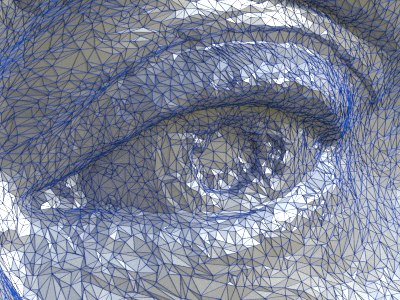
\includegraphics[width=\textwidth]{process_f02_01}}
        \caption{}\label{fig:process_original_scan}
    \end{subfigure}
    \hfill
    \begin{subfigure}[t]{0.195\textwidth}
        \inlinelabel{b}{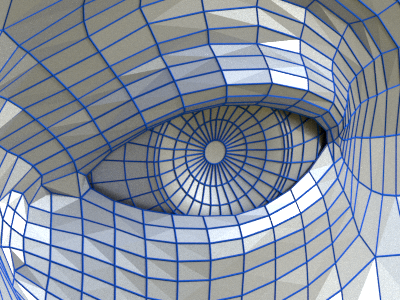
\includegraphics[width=\textwidth]{process_f02_02}}
        \caption{}\label{fig:process_retopo}
    \end{subfigure}
    \hfill
    \begin{subfigure}[t]{0.195\textwidth}
        \inlinelabel{c}{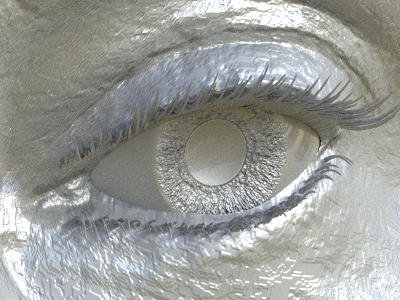
\includegraphics[width=\textwidth]{process_f02_03}}
        \caption{}\label{fig:process_displaced_subdiv}
    \end{subfigure}
    \hfill
    \begin{subfigure}[t]{0.195\textwidth}
        \inlinelabel{d}{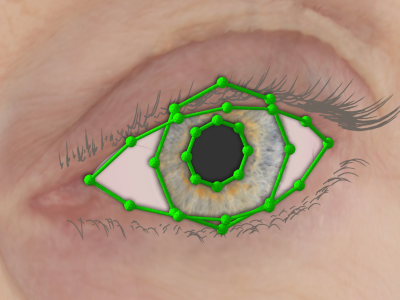
\includegraphics[width=\textwidth]{process_f02_04}}
        \caption{}\label{fig:process_ldmks}
    \end{subfigure}
    \hfill
    \begin{subfigure}[t]{0.195\textwidth}
        \inlinelabel{e}{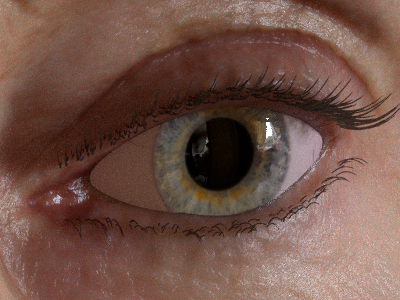
\includegraphics[width=\textwidth]{process_f02_05}}
        \caption{}\label{fig:process_final_render}
    \end{subfigure}
    \par\vspace{-28pt}
    \caption{An overview of our model preparation process: Dense 3D head scans (1.4 million polygons) \subref{fig:process_original_scan} are first retopologised into an optimal form for animation (9,005 polygons) \subref{fig:process_retopo}. High resolution skin surface details are restored by displacement maps \subref{fig:process_displaced_subdiv}, and 3D iris and eyelid landmarks are annotated manually \subref{fig:process_ldmks}. A sample rendering is shown \subref{fig:process_final_render}.}
    \label{fig:process}
\end{figure*}